\chapter{Appendix}
\label{appendix}

\qquad The same dataset has been also projected onto 2D plane, as illustrated in the figure \ref{metrics-pca-13-to-2}.

\begin{figure}[htb]
	\centering
	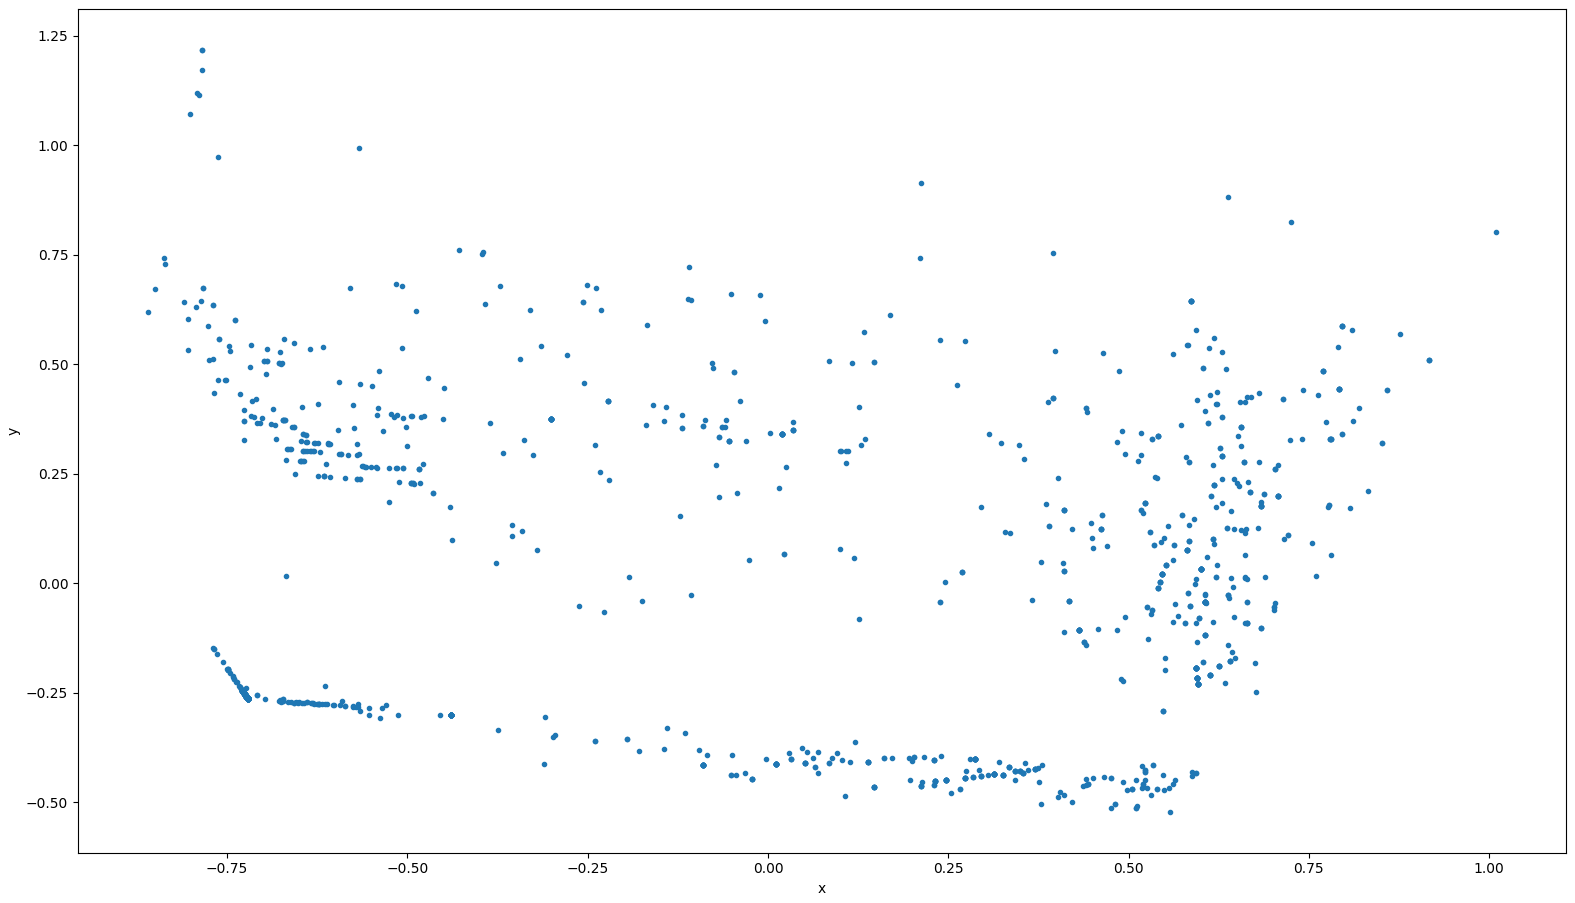
\includegraphics[width=\linewidth]{figs/metrics-pca-13-to-2.png}
	\caption{Visualisation of loop metrics dataset (13-dimensional metric vectors have been projected onto 2d space thanks to PCA algorithm) - blue dots correspond to metric values on single loops.}
	\label{metrics-pca-13-to-2}
\end{figure}

\begin{figure}[h]
	\centering
	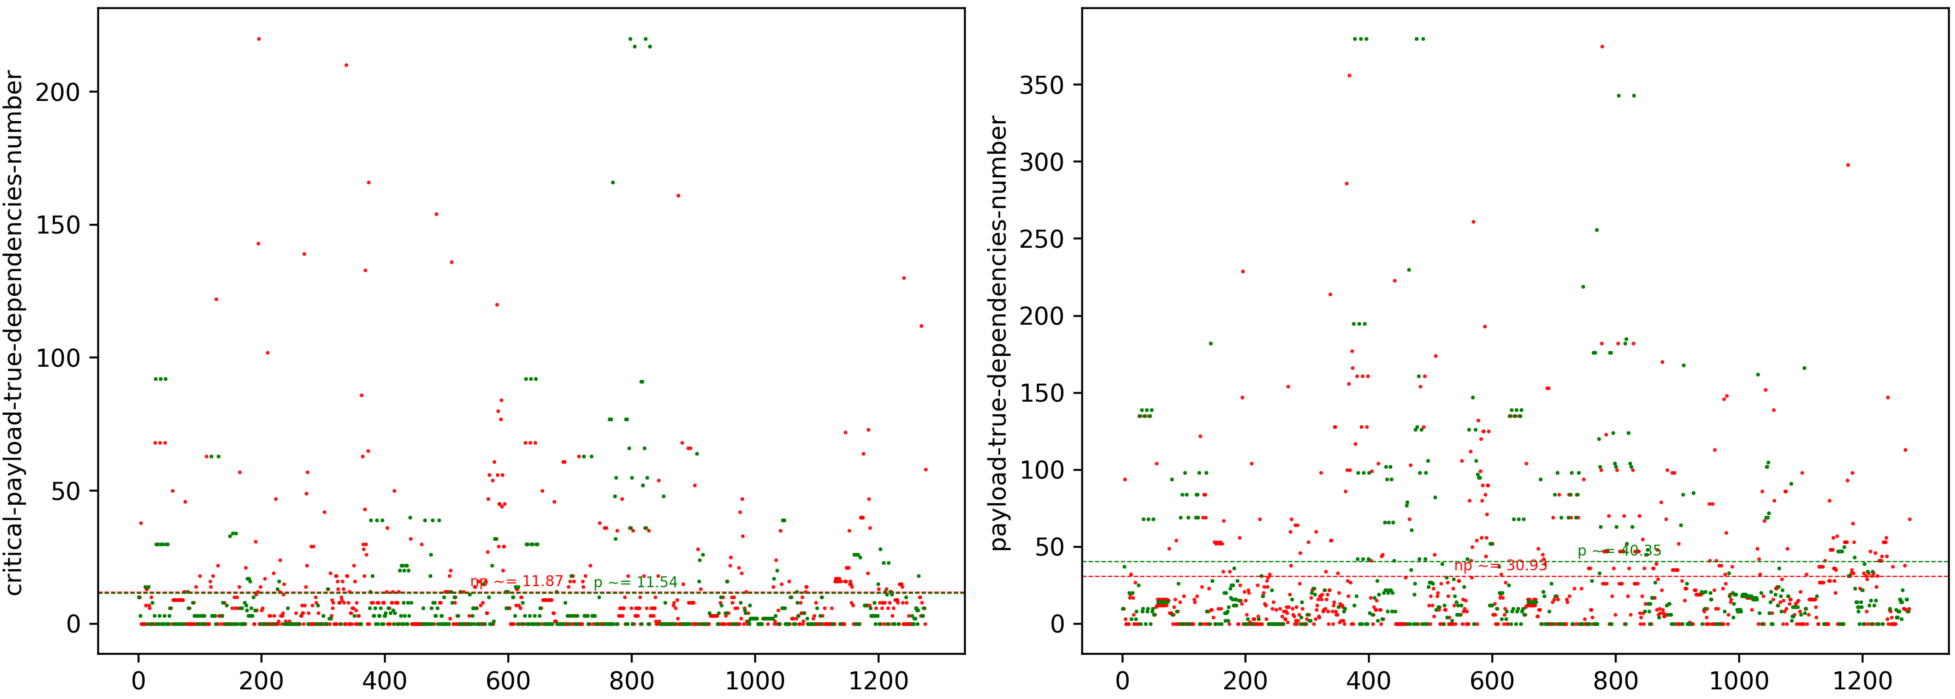
\includegraphics[width=\linewidth]{figs/loop-dependencies-number-1.png}
	\caption{\textit{Critical payload true dependencies number} metric on the left and \textit{payload true dependencies number} metric on the right. Red and green dots represent loops, which have not/have been parallelized by ICC compiler correspondingly.}
	\label{loop-dependencies-number-1}
\end{figure}

\begin{figure}[h]
	\centering
	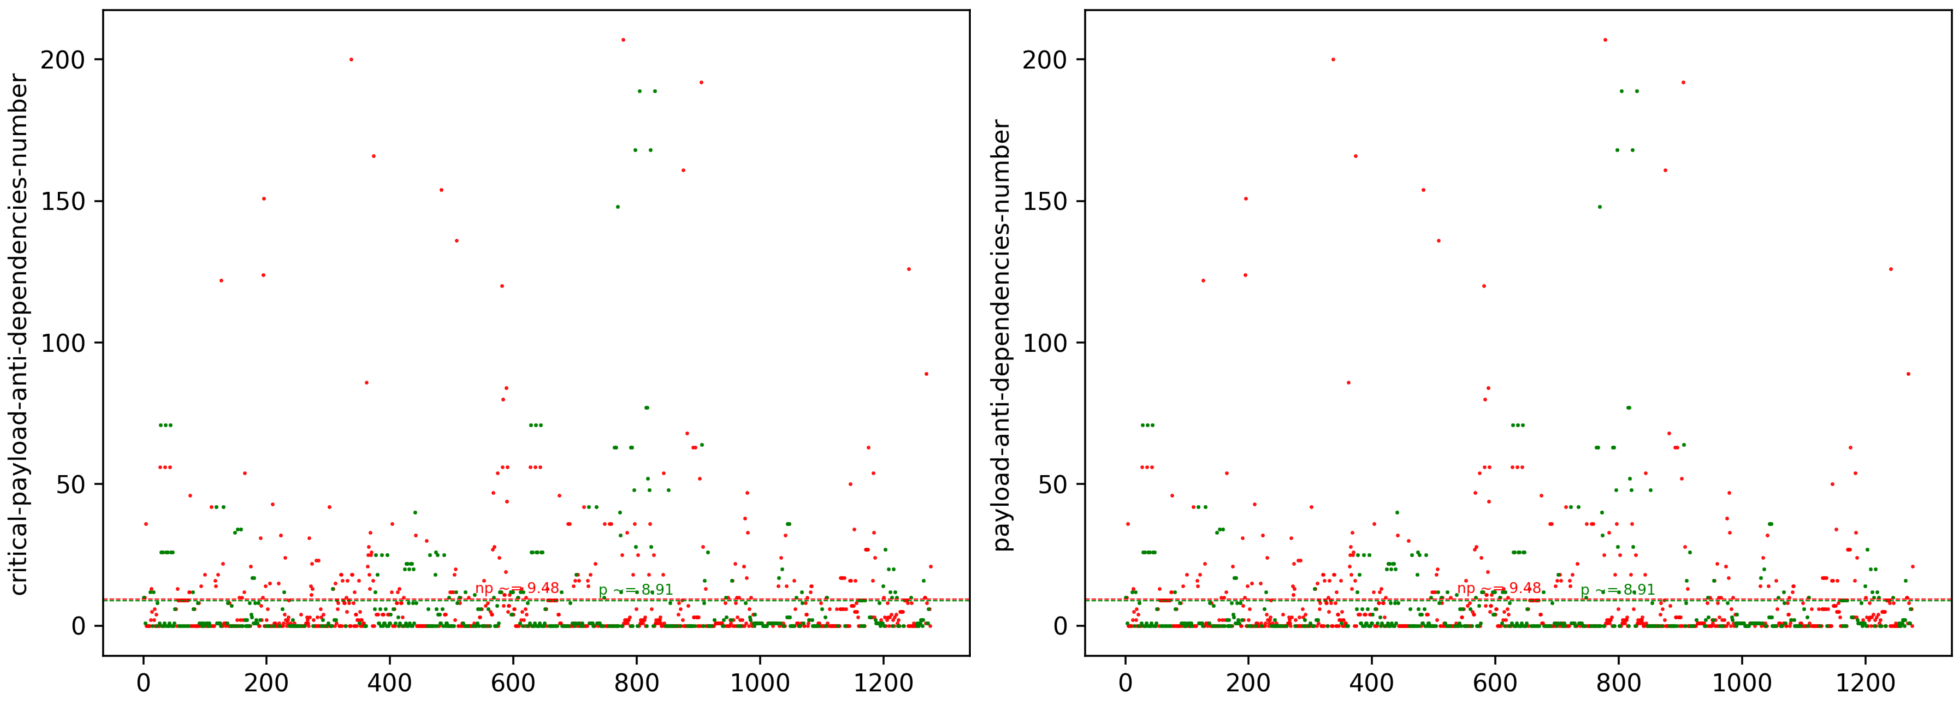
\includegraphics[width=\linewidth]{figs/loop-dependencies-number-2.png}
	\caption{\textit{Critical payload anti dependencies number} metric on the left and \textit{payload anti dependencies number} metric on the right. Red and green dots represent loops, which have not/have been parallelized by ICC compiler correspondingly.}
	\label{loop-dependencies-number-2}
\end{figure}